% Author: Taejin Hwang
% Email: taejin@berkeley.edu

\qns{Transient analysis}

We have taken a look at how to take a \textbf{system} of differential equations, convert it the following \textbf{vector} differential equation.

\begin{equation}\label{eq:vec}
\ddt{}{t} \vec{x}(t) = A \vec{x}(t) + \vec{b}(t)
\end{equation}

With initial condition $\vec{x}(0) = \begin{bmatrix} x_1(0) \\ x_2(0) \end{bmatrix}$

We made the observation that we could convert our differential equation from standard coordinates into coordinates using a basis entirely made up of $A$'s eigenvectors, in which the linear operator of $A$ became a diagonal matrix, $D,$ where the diagonal entires are the eigenvalues of $A.$

\begin{equation}\label{eq:diag}
\ddt{}{t} \vec{z}(t) = D \vec{z}(t) + \widetilde{\vec{b}}(t)
\end{equation}

With initial condition $\vec{z}(0) = \begin{bmatrix} z_1(0) \\ z_2(0) \end{bmatrix}$

In this problem, we will analyze the different types of transient responses that a system can have, based on the eigenvalues of $A.$

Consider the following RLC Circuit with $V_{s} = \SI{4}{\volt}, \ R = \SI{4}{\ohm}, \ L = \SI{1}{\henry}, \ C = \SI{1/3}{\farad}$ the capacitor is initially uncharged and there is no current flowing in the circuit at $t = 0.$

\qns{RLC circuit \#1}
\qcontributor{Varun Mishra}

In this question, we will take a look at an electrical systems described by second order differential equations and analyze it using the phasor domain. Consider the circuit below where $R=3 \text{k}\Omega$, $L=1\mbox{mH}$, $C=100$nF, and $V_{\text{s}}=5\cos(1000t+\frac{\pi}{4})$:

\begin{center}
		\begin{circuitikz}[scale=0.8]
			\draw (0,4) 
			to [sV, l= $V_s$] (0,0)
			(0,4)
			to [R = $R$,v=$V_R$] (4,4)
			to [L = $L$,v=$V_L$,i=$i(t)$] (8,4)
			to [short] (10,4)
			to [C = $C$,v=$V_{\text{out}}$] (10,0)	
			to [short] (0,0);
		\end{circuitikz}
	\end{center}
\begin{enumerate}
	
    \qitem What are the impedances of the resistor, inductor and capacitor, $Z_R$, $Z_L$, and $Z_C$?
    
\sol{
\begin{align*}
\intertext{The impedance of a resistor is the same as its resistance}
Z_R &= 3000\Omega 
\intertext{We can find the frequency of the circuit by looking at $V_{\text{s}}$. The form of a cosine function is $A\cos(\omega t+\phi )$ where $A$ is amplitude, $\omega$ is frequency, and $\phi$ is phase. In this case, the frequency is $1000 \frac{\text{rad}}{\text{s}}$}
Z_L &= j\omega L = j1000*10^{-3}= j1 \Omega \\
Z_C &= \frac{1}{j\omega C} = \frac{1}{j1000*10^{-7}} =-j10^4 \Omega
\end{align*}

}  
\qitem Solve for $\widetilde{V}_{\text{out}}$ in phasor form.

\sol{
\begin{align*}
\intertext{converting $V_{\text{s}}$ into phasor form, we have}
\widetilde{V}_{\text{s}} &= \frac{1}{2} |A|e^{j\phi} = \frac{5}{2}e^{j\frac{\pi}{4}} 
\intertext{The circuit given is a voltage divider. Since impedances act like resistors, we can use the same equation as the resistive voltage divider.}
\widetilde{V}_{\text{out}} = \widetilde{V}_{\text{s}}\frac{Z_C}{Z_R+Z_L+Z_C}&= \widetilde{V}_{\text{s}}*\big|\frac{Z_C}{Z_R+Z_L+Z_C}\big|e^{j*\angle\big(\frac{Z_C}{Z_R+Z_L+Z_C}\big)} \tag{1} \\ 
\intertext{We can solve for the magnitude and angle of the divider using}
\big|\frac{Z_C}{Z_R+Z_L+Z_C}\big|&=\frac{|Z_C|}{|Z_R+Z_L+Z_C|}=\frac{10^4}{\sqrt{3000^2+(1-10^4)^2}} = 0.958 \\
\angle\big(\frac{Z_C}{Z_R+Z_L+Z_C}\big)&= \angle(Z_C)-\angle(Z_R+Z_L+Z_C)=\text{atan2}\Big(\frac{\mathfrak{Im}(Z_C)}{\mathfrak{Re}(Z_C)}\Big)-\text{atan2}\Big(\frac{\mathfrak{Im}(Z_R+Z_L+Z_C)}{\mathfrak{Re}(Z_R+Z_L+Z_C)}\Big) \\
\angle\big(\frac{Z_C}{Z_R+Z_L+Z_C}\big)&=-0.2915 \text{ rad}
\intertext{Plugging back into (1)}
\widetilde{V}_{\text{out}}&=\frac{5}{2}e^{j\frac{\pi}{4}}*0.958e^{-j0.2915}= 2.395 e^{j0.494}
\end{align*}
}
    
   
 \qitem Solve for the transfer function $H(\omega)=\frac{\widetilde{V}_{\text{out}}}{\widetilde{V}_{\text{s}}}$
 
  Leave your answer in terms of $R$, $L$, $C$, and $\omega$.
 
\sol{
\begin{align*}
\intertext{Looking back at equation (1)}
\widetilde{V}_{\text{out}} &= \widetilde{V}_{\text{s}}\frac{Z_C}{Z_R+Z_L+Z_C}
\intertext{Rearranging we get}
H(\omega)&=\frac{\widetilde{V}_{\text{out}}}{\widetilde{V}_{\text{s}}}= \frac{Z_C}{Z_R+Z_L+Z_C}=\frac{\frac{1}{j\omega C}}{R+j\omega L+\frac{1}{j\omega C}} \\
H(\omega) &= \frac{1}{LC(j\omega)^2+jRC\omega+1}
\end{align*}
}
  
\qitem Solve for the current $i(t)$

    \sol{
    \begin{align*}
    \widetilde{i}&=\frac{\widetilde{V}_{\text{s}}}{Z_R+Z_L+Z_C} = \frac{|\widetilde{V}_{\text{s}}|}{|Z_R+Z_L+Z_C|}e^{j\big(\angle \widetilde{V}_{\text{s}}- \angle (Z_R+Z_L+Z_C)\big)} = 2.395*10^{-4}e^{j2.0647}
    \intertext{Going back to the time domain:}
    i(t)&=4.790*10^{-4}\cos(1000t+2.0647) \text{ A}
    \end{align*}
    }

\qitem What is $V_{\text{out}}$ in the time domain?

\sol{
\begin{align*}
% V_{\text{out}}(t)&= \mathfrak{Re}(\widetilde{V}_{\text{out}}e^{j\omega t})
% \intertext{Using Euler's formula, we can say}
% \widetilde{V}_{\text{out}}e^{j\omega t} &= |\widetilde{V}_{\text{out}}|\big(\cos(\omega t+\angle \widetilde{V}_{\text{out}})+j\sin(\omega t+\angle \widetilde{V}_{\text{out}})\big) 
% \intertext{Taking the real part, we get}
% \mathfrak{Re}(\widetilde{V}_{\text{out}}e^{j\omega t}) &= |\widetilde{V}_{\text{out}}|\cos(\omega t+\angle \widetilde{V}_{\text{out}}) \\
V_{\text{out}}(t)&= 4.79\cos(1000t+0.494) \text{ V}
\end{align*}
}

\end{enumerate}



\qitem \textbf{Step 1: Define state variables}

\meta{
  The same process can be done by defining $x_{1}(t) = V_{out}(t)$ and $x_{2}(t) = \ddt{V_{out}(t)}{t}.$ Make sure students are familiar with how to handle both cases. We choose $i(t)$ here since $i(t) = C \ddt{V_{out}(t)}{t}.$
}

When setting up a system of differential equations, it is important to always start by definining a state variable to create a vector differential equation. For the sake of this question, we will define our state variable as:

\begin{equation}
\vec{x}(t) =  \begin{bmatrix} x_{1}(t) \\ x_{2}(t) \end{bmatrix} = \begin{bmatrix} V_\text{c}(t) \\ i(t) \end{bmatrix}
\end{equation}

\qitem \textbf{Step 2: Write out a system of differential equations}

The next step is to set up a system of differential equations using the individual state variables that you defined in the previous part.

How can you write out a system of differential equations in terms of your state variables $x_{1}(t) = V_\text{c}(t)$ and $x_{2}(t) = i(t)?$

\sol {
	The voltage-current relationship of a capacitor tells us that
	$$i(t) = C \ddt{}{t} V_\text{c}(t)$$
	This can equivalently be written as:
	$$\ddt{}{t} x_{1}(t) = \frac{1}{C} x_{2}(t)$$
	The voltage-current relationship of an inductor tells us that
	$$V_{L}(t) = L \ddt{}{t} i(t)$$
	So we see that
	$$\ddt{}{t} i(t) = \frac{1}{L} V_{L}(t)$$
	However, $V_{L}(t)$ is not a state variable, meaning we must find a way to express $V_{L}(t)$ in terms of our state variables. Therefore by using KVL:
	$$V_{s} = V_{R}(t) + V_{\text{c}}(t) + V_{L}(t)$$
	Which implies that
	$$V_{L}(t) = V_{s} - V_{R}(t) - V_{\text{c}}(t) = V_{s} - i(t) \cdot R - V_{\text{c}}(t)$$
	Therefore:
	$$\ddt{}{t} i(t) = \frac{1}{L} \big( V_{s} - i(t) \cdot R - V_{\text{c}}(t) \big)$$
	As state variables:
	$$\ddt{}{t} x_{2}(t) = -\frac{1}{L} x_{1}(t) - \frac{R}{L} x_{2}(t) + \frac{1}{L} V_{s}$$

  The initial conditions must be:
  \begin{gather*}
  x_{1}(0) = 0 \\
  x_{2}(0) = 0
  \end{gather*}
  Since the capacitor starts off uncharged, and the voltage across the capacitor cannot change instantaneously.
  Similarly, the current across the inductor cannot change instantenously, so the current through the inductor cannot change instantaneously.
}

\qitem \textbf{Step 3: Turn this system of differential equations into a vector differential equation}

Given the system of differential equations you wrote in the previous part, the next step is to create a vector differential equation of the form:

\begin{equation}
\ddt{}{t} \vec{x}(t) = A \vec{x}(t) + \vec{b}
\end{equation}

\sol {
	Taking the derivative of $\vec{x}(t)$ we get:
	$$\ddt{}{t} \vec{x}(t) = \begin{bmatrix} \ddt{}{t} x_{1}(t) \\ \ddt{}{t} x_{2}(t) \end{bmatrix} = 
	\begin{bmatrix} \frac{1}{C} x_{2}(t) \\ -\frac{1}{L} x_{1}(t) - \frac{R}{L} x_{2}(t) + \frac{V_s}{L} \end{bmatrix}$$
	We can write this in matrix-vector form:
	$$\ddt{}{t} \vec{x}(t) = \begin{bmatrix} 0 & \frac{1}{C} \\ -\frac{1}{L} & - \frac{R}{L} \end{bmatrix} 
	\begin{bmatrix} x_{1}(t) \\  x_{2}(t) \end{bmatrix} + \begin{bmatrix} 0 \\ \frac{V_s}{L} \end{bmatrix} $$
	So we can see that:
	\begin{gather*}
	A = \begin{bmatrix} 0 & \frac{1}{C} \\ -\frac{1}{L} & - \frac{R}{L} \end{bmatrix} 
	\text{ and  }
	\vec{b} = \begin{bmatrix} 0 \\ \frac{V_s}{L} \end{bmatrix}
	\end{gather*}
  With initial condition $\vec{x}(0) = \begin{bmatrix} 0 \\ 0 \end{bmatrix}$
  Numerically the values will be:
  \begin{gather*}
  A = \begin{bmatrix} 0 & 3 \\ -1 & - 4 \end{bmatrix} 
  \text{ and  }
  \vec{b} = \begin{bmatrix} 0 \\ 4 \end{bmatrix}
  \end{gather*}
}

\qitem \textbf{Step 4: Find the coordinate transformation to the eigenbasis}

The next step is to find a change of variables to the a basis made up of eigenvectors.
Remember that this is equivalent to finding the eigenvectors and eigenvalues of the matrix $A.$ 
Order the eigenvalues from smallest to largest.

\sol{
	To find the eigenvalues of $A,$ we try to solve for $\lambda$ such that $\text{det} (A - \lambda I) = 0.$
	$$\text{det} (A - \lambda I) = \text{det} \Big( \begin{bmatrix} - \lambda & \frac{1}{C} \\ -\frac{1}{L} & - \frac{R}{L} - \lambda \end{bmatrix} \big) = (- \lambda) (-\frac{R}{L} - \lambda) + \frac{1}{LC} = \lambda^{2} + \frac{R}{L} \lambda + \frac{1}{LC} $$
	We can solve for $\lambda$ by using the quadratic formula:
	$$\lambda = -\frac{R}{2L} \pm \sqrt{\big(\frac{R}{2L} \big)^2 - \frac{1}{LC}}$$
	To find the eigenvectors of $A,$ we look at the null-space of $A - \lambda I.$
	$$A - \lambda_{1} I = \begin{bmatrix} - \lambda_{1} & \frac{1}{C} \\ -\frac{1}{L} & - \frac{R}{L} - \lambda_{1} \end{bmatrix}$$
	A basis for the null-space of $A - \lambda_{1} I$ is: 
	$$\vec{v}_{1} = \begin{bmatrix} 1 \\ \lambda_1 C \end{bmatrix}$$
	A basis for the null-space of $A - \lambda_{2} I$ can be similarly calculated as:
	$$\vec{v}_{2} = \begin{bmatrix} 1 \\ \lambda_2 C \end{bmatrix}$$
  Numerically, the eigenvalues are:
  \begin{gather*}
  \lambda_{1} = -3, \  \lambda_{2} = -1
  \end{gather*}
  Numerically, the basis will be:
  \begin{gather*}
  \vec{v}_{1} = \begin{bmatrix} 1 \\ -1 \end{bmatrix}, \ \vec{v}_{2} = \begin{bmatrix} 1 \\ -\frac{1}{3} \end{bmatrix}
  \end{gather*}
}

\qitem \textbf{Step 5: Convert the system from standard to eigenbasis coordinates}

Since we found our eigenbasis basis $S = \{ \vec{v_1}, \vec{v_2} \},$ we will define the change of coordinates matrix from S-coordinates to standard basis coordinates as:

$$\vec{z} = \begin{bmatrix} z_1 \\ z_2 \end{bmatrix} {  ,  } \ \ \vec{x} = z_1 \vec{v_1} + z_2 \vec{v_2} \text{  and  } V = \begin{bmatrix} 1 & 1 \\ \lambda_1 C & \lambda_2 C \end{bmatrix} \text {  s.t.  } \vec{x} = V \vec{z} $$ 

How can we write out the differential equation using eigenbasis coordinates, or in terms of $\vec{z}(t)?$

\begin{equation}
	\ddt{}{t} \vec{z}(t) = D \vec{z}(t) + \widetilde{\vec{b}}
\end{equation}

\sol {
  We've defined the change of coordinates from eigenbasis to standard coordinates as $\vec{x} = V \vec{z}.$
  The vector differential equation that we currently have is:

  \begin{equation}
  	\ddt{}{t} \vec{x}(t) = A \vec{x}(t) + \vec{b}(t)
  \end{equation}

  We can substitute $\vec{x} = V \vec{z}$ to get:

  \begin{equation}
  	\ddt{}{t} V \vec{z}(t) = A V \vec{z}(t) + \vec{b}(t)
  \end{equation}

  Since we have a derivative of a linear combination, this is the same as a linear combination of the derivatives:

  \begin{equation}
  	V \ddt{}{t} \vec{z}(t) = A V \vec{z}(t) + \vec{b}(t)
  \end{equation}

  Then after applying $V^{-1}$ to both sides, we get:

  \begin{equation}
  	\ddt{}{t} \vec{z}(t) = V^{-1} A V \vec{z}(t) + V^{-1} \vec{b}(t)
  \end{equation}

  Therefore, we see that $D = V^{-1} A V$ and $\widetilde{\vec{b}} = V^{-1} \vec{b}.$

  We know the matrix $V^{-1} A V$ is diagonal with the eigenvalues of $A$ and we can compute $V^{-1}$
  $$V^{-1} = \frac{1}{\lambda_{2} C - \lambda_{1} C} \begin{bmatrix} \lambda_{2} C & -1 \\ -\lambda_{1} C & 1 \end{bmatrix}$$

  Therefore we can calculate $\widetilde{\vec{b}}$ as:
  $$V^{-1} \vec{b}(t) = \frac{1}{\lambda_{2} C - \lambda_{1} C} \begin{bmatrix} \lambda_{2} C & -1 \\ -\lambda_{1} C & 1 \end{bmatrix} \begin{bmatrix} 0 \\ \frac{V_s}{L} \end{bmatrix} = \frac{1}{\lambda_{2} C - \lambda_{1} C} \begin{bmatrix} -\frac{V_s}{L} \\ \frac{V_s}{L} \end{bmatrix} = \begin{bmatrix} -\frac{V_s}{LC(\lambda_{2} - \lambda_{1})} \\ \frac{V_s}{LC(\lambda_{2} - \lambda_{1})} \end{bmatrix}  $$

  Lastly, the initial condition will be:
  $$\vec{z}(0) = V^{-1} \vec{x}(0) = \begin{bmatrix} 0 \\ 0 \end{bmatrix}$$

  Numerically, the system of differential equations should be:
  \begin{equation}
  \ddt{}{t} \vec{z}(t) = \begin{bmatrix} -3 & 0 \\ 0 & -1 \end{bmatrix} \vec{z}(t) + \begin{bmatrix} -6 \\ 6 \end{bmatrix}
  \end{equation}
}

\qitem \textbf{Step 6: Solve the differential equation in eigenbasis coordinates}

We can uncouple our system of differential equations into a pair of first-order scalar differential equations:
  \begin{gather*}
    \ddt{}{t} z_{1}(t) = \lambda_1 z_{1}(t) - \frac{V_s}{LC(\lambda_{2} - \lambda_{1})} \\
    \ddt{}{t} z_{2}(t) = \lambda_2 z_{2}(t) + \frac{V_s}{LC(\lambda_{2} - \lambda_{1})}
  \end{gather*}

With initial condition $\vec{z}(0) = \begin{bmatrix} 0 \\ 0 \end{bmatrix}.$
How can we solve these differential equations?

\sol{
  They are first-order differential equations with a constant input!

  Recall that for a first order, differential equation with constant input:

  \begin{equation} \label{eq:h}
    \ddt{x(t)}{t} = \lambda x(t) + u
  \end{equation}

  With initial condition $x(0) = x_0,$ the particular solution to the equation for $t \geq 0$, $x_p(t),$ was uniquely determined as:
  \begin{equation} \label{eq:hs}
  x_p(t) = x(0) e^{\lambda t} + \frac{u}{\lambda} (e^{\lambda t} - 1)
  \end{equation}

  Therefore the solutions will be:
  \begin{gather*}
    z_{1}(t) = -\frac{V_{s}}{LC(\lambda_{2} - \lambda_{1})\lambda_1} \big(e^{\lambda_{1}t} - 1 \big) \\
    z_{2}(t) = \frac{V_{s}}{LC(\lambda_{2} - \lambda_{1})\lambda_2} \big(e^{\lambda_{2}t} - 1 \big)
  \end{gather*}

  Numerically they will be:
  \begin{gather*}
    z_{1}(t) = 2(e^{-3t} - 1) = 2e^{-3t} - 2\\
    z_{2}(t) = -6(e^{-t} - 1) = -6e^{-t} + 6
  \end{gather*}

  Therefore the solution in vector form will be:
  \begin{equation}
  \vec{z}(t) = \begin{bmatrix} z_{1}(t) \\ z_{2}(t) \end{bmatrix} =
  \begin{bmatrix} -\frac{V_s(e^{\lambda_{1} t} - 1)}{LC(\lambda_{2} - \lambda_{1})\lambda_{1}} \\ 
  \frac{V_s(e^{\lambda_{2} t} - 1)}{LC(\lambda_{2} - \lambda_{1})\lambda_{2}} \end{bmatrix} = 
  \begin{bmatrix} 2e^{-3t} - 2 \\ -6e^{-t} + 6
  \end{bmatrix}
  \end{equation}
}

\qitem \textbf{Step 7: Convert the solutions back into standard basis coordinates}

We have solved our differential equation in S-basis or $z_i$ coordinates.
However, our original differential equation was in terms of standard basis, or $x_i$ coordinates.
Convert the solutions that are currently in $z_i$ coordinates to a solution in $x_i$ coordinates.
Try to sketch the solution $V_{out}(t)$ as well.

\sol {
  The relationship between $\vec{x}$ and $\vec{z}$ is $\vec{x} = V \vec{z}.$
  Therefore we see that the solution to our differential equation in $x_i$ coordinates is:
  $$\vec{x}(t) = \begin{bmatrix} 1 & 1 \\ \lambda_1 C & \lambda_2 C \end{bmatrix} \vec{z}(t) = 
  \begin{bmatrix} -\frac{V_s(e^{\lambda_{1} t} - 1)}{LC(\lambda_{2} - \lambda_{1})\lambda_{1}} + 
  \frac{V_s(e^{\lambda_{2} t} - 1)}{LC(\lambda_{2} - \lambda_{1})\lambda_{2}} \\ 
  -\frac{V_s(e^{\lambda_{1} t} - 1)}{L(\lambda_{2} - \lambda_{1})} + 
  \frac{V_s(e^{\lambda_{2} t} - 1)}{L(\lambda_{2} - \lambda_{1})} \end{bmatrix}   
  = \begin{bmatrix} -\frac{\lambda_{2} V_s (e^{\lambda_{1} t} - 1)}{LC(\lambda_{2} - \lambda_{1})\lambda_{1}\lambda_{2}} + 
  \frac{\lambda_{1} V_s (e^{\lambda_{2} t} - 1)}{LC(\lambda_{2} - \lambda_{1})\lambda_{1} \lambda_{2}} \\ 
  \frac{V_s(e^{\lambda_{2} t} - e^{\lambda_{1} t} + 1 - 1)}{L(\lambda_{2} - \lambda_{1})} \end{bmatrix} 
  $$

  A crucial realization that we can make is that $\lambda_1 \lambda_2 = \frac{1}{LC}$ therefore:
  $$\vec{x}(t) = \begin{bmatrix} \frac{-\lambda_{2} V_s (e^{\lambda_{1} t} - 1) + \lambda_{1} V_s (e^{\lambda_{2} t} - 1)}{\lambda_{2} - \lambda_{1}} \\ 
  \frac{V_s e^{\lambda_{2} t}}{L(\lambda_{2} - \lambda_{1})} - \frac{V_s e^{\lambda_{1} t}}{L(\lambda_{2} - \lambda_{1})} \end{bmatrix}
  = \begin{bmatrix} \frac{-\lambda_{2} V_s e^{\lambda_{1} t}}{\lambda_{2} - \lambda_{1}} + \frac{\lambda_{1} V_s e^{\lambda_{2} t}}{\lambda_{2} - \lambda_{1}} + \frac{\lambda_{2} V_s}{\lambda_{2} - \lambda_{1}} - \frac{\lambda_{1} V_s}{\lambda_{2} - \lambda_{1}} \\
  \frac{V_s e^{\lambda_{2} t}}{L(\lambda_{2} - \lambda_{1})} - \frac{V_s e^{\lambda_{1} t}}{L(\lambda_{2} - \lambda_{1})} \end{bmatrix}
  = \begin{bmatrix} \frac{-\lambda_{2} V_s e^{\lambda_{1} t}}{\lambda_{2} - \lambda_{1}} + \frac{\lambda_{1} V_s e^{\lambda_{2} t}}{\lambda_{2} - \lambda_{1}} + V_s \\
  \frac{V_s e^{\lambda_{2} t}}{L(\lambda_{2} - \lambda_{1})} - \frac{V_s e^{\lambda_{1} t}}{L(\lambda_{2} - \lambda_{1})} \end{bmatrix}
  $$ 

  Since we were initially solving for $x_{1}(t) = V_{\text{c}}(t) = V_{out}(t),$ our final result is:
  $$V_{out}(t) = \frac{-\lambda_{2} V_s e^{\lambda_{1} t}}{\lambda_{2} - \lambda_{1}} + \frac{\lambda_{1} V_s e^{\lambda_{2} t}}{\lambda_{2} - \lambda_{1}} + V_s$$

  Numerically, it will look like:
  $$\vec{x}(t) = \begin{bmatrix} 1 & 1 \\ -1 & -\frac{1}{3} \end{bmatrix} \vec{z}(t) = 
  \begin{bmatrix} 2e^{-3t} - 6e^{-t} + 4 \\  -2e^{-3t} + 2e^{-t} \end{bmatrix}$$

  So $x_{1}(t) = V_{\text{c}}(t) = V_{out}(t)$
  $$V_{out}(t) = 2e^{-3t} - 6e^{-t} + 4$$

  \begin{figure}[!ht]
    \centering
    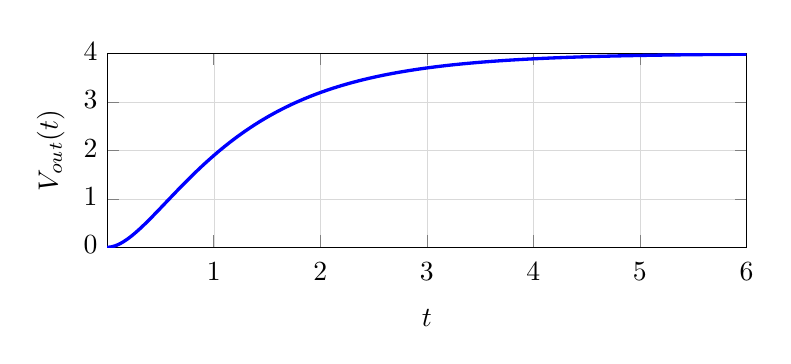
\begin{tikzpicture}[
        declare function={
          od(\x)= 2*exp(-3*\x) - 6*exp(-\x) + 4;
        }
    ]
    \begin{axis}[
      typeset ticklabels with strut,
      ymin=0, ymax=4, ylabel=$V_{out}(t)$, xlabel=$t$,
      xmin = 0, xmax = 6, xtick = {1,2,3,4,5,6}, domain=0:6, 
      grid=both, grid style={line width=.1pt, draw=gray!30},
      width=\textwidth * 0.8,
      height=\textwidth / 3,
      samples = 800
    ]
    \addplot [blue,very thick] {od(x)};
    \end{axis}
    \end{tikzpicture}
  \end{figure}
}

\qitem \textbf{Step 8: Analyze the eigenvalues}

The eigenvalues in step 4 were calculated using the quadratic formula: 
$$\lambda = -\frac{R}{2L} \pm \sqrt{\big(\frac{R}{2L} \big)^2 - \frac{1}{LC}}$$
When are the eigenvalues of $A$ real, and when are they imaginary?

\sol {
  The value of $(\frac{R}{L})^2 - \frac{4}{LC}$ will determine whether $\lambda$ is real or complex. 
  \begin{itemize}
  \item When the value of $(\frac{R}{L})^2 - \frac{4}{LC}$ is greater than or equal to zero, $\lambda$ must be real. 
  This occurs when $R > 2 \sqrt{\frac{L}{C}}.$
  \item When the value of $(\frac{R}{L})^2 - \frac{4}{LC}$ is negative, $\lambda$ must be complex. 
  This occurs when $R < 2 \sqrt{\frac{L}{C}}.$
  \item If the square root term is equal to 0, then there will be one distinct real eigenvalue. 
  We will discuss this case in more depth as a special part.
  \end{itemize}
}

\qitem \textbf{Step 9: The complex response}
We will now take a look at the case when the eigenvalues are complex. Let $R = \SI{2}{\ohm}, \ L = \SI{1}{\henry}, \ C = \SI{1/2}{\farad}.$ Compute the eigenvalues, and solve for the differential equation in a similar manner to the previous parts. 
Then try to sketch the response $V_{out}(t).$

\sol {
  We can compute our eigenvalues as $\lambda_{1} = -1 - j$ and $\lambda_{2} = -1 + j.$
  The system of differential equations is the same except $u_{1} = -\frac{V_{s}}{LC(\lambda_{2} - \lambda_{1})}$ and $u_{2} = \frac{V_{s}}{LC(\lambda_{2} - \lambda_{1})}$
  \begin{gather*}
    \ddt{}{t} z_{1}(t) = \lambda_{1} z_{1}(t) + 4j \\
    \ddt{}{t} z_{2}(t) = \lambda_{2} z_{2}(t) - 4j
  \end{gather*}
  With unique solutions: 
  \begin{gather*}
    z_{1}(t) = z(0) e^{\lambda_{1} t} + \frac{4j}{\lambda_{1}} (e^{\lambda_{1} t} - 1)  \\
    z_{2}(t) = z(0) e^{\lambda_{2} t} + \frac{-4j}{\lambda_{2}} (e^{\lambda_{2} t} - 1)
  \end{gather*}
  Using Euler's formula, we see that:
  \begin{gather*}
    e^{\lambda_{1} t} = e^{(-1 - j)t} = e^{-t} (\cos (t) - j \sin(t)) \\
    e^{\lambda_{2} t} = e^{(-1 + j)t} = e^{-t} (\cos (t) + j \sin(t)) 
  \end{gather*}
  So plugging back into $z_{i}(t),$ we get:
  \begin{gather*}
    z_{1}(t) = \frac{4j}{-1 - j} (e^{-t} \cos(t) - j e^{-t} \sin(t) - 1) = (-2 - 2j) (e^{-t} \cos(t) - j e^{-t} \sin(t) - 1)  \\
    z_{2}(t) = \frac{-4j}{-1 + j} (e^{-t} \cos(t) + j e^{-t} \sin(t) - 1) = (-2 + 2j) (e^{-t} \cos(t) + j e^{-t} \sin(t) - 1)
  \end{gather*}
  Simplifying yields:
  $$z_{1}(t) = (-2 - 2j) e^{-t} \cos(t) + (-2 - 2j) e^{-t} \sin(t) + (2 + 2j)$$
  $$z_{2}(t) = (-2 + 2j) e^{-t} \cos(t) + (-2 - 2j) e^{-t} \sin(t) + (2 - 2j) $$
  Converting back into $x_{i}$ coordinates, we see that:
  $$\vec{x}(t) = \begin{bmatrix} 1 & 1 \\ -\frac{1}{2}-\frac{j}{2} & -\frac{1}{2}+\frac{j}{2} \end{bmatrix} \vec{z}(t) = 
  \begin{bmatrix} -4 e^{-t} \cos(t) -4 e^{-t} \sin(t) + 4 \\ 4e^{-t} \sin(t) \end{bmatrix}
  $$
  The graph of this function will have an exponential rise with oscillations at the same time.
  For this specific graph, the oscillations aren't as visible, but if we modified our capacitor value to be smaller, then $|\mathfrak{Im}(\lambda)|$ would be larger, and there will be more oscillations. 
  The graphs for $\mathfrak{Re}(\lambda) = -1$ are plotted below.

  \begin{figure}[!h]
    \centering
    \begin{tikzpicture}[
        declare function={
          ud(\x)= -4* exp(-\x) * cos(deg(\x)) -4* exp(-\x) * sin(deg(\x)) + 4;
        }
    ]
    \begin{axis}[
      typeset ticklabels with strut,
      ymin=0, ymax=6, ytick={0, 2, 4, 6}, ylabel=$V_{out}(t)$, xlabel=$t$,
      xmin = 0, xmax = 6, xtick = {1,2,3,4,5,6}, domain=0:6, 
      grid=both, grid style={line width=.1pt, draw=gray!30},
      width=\textwidth * 0.8,
      height=\textwidth / 4.2,
      samples = 1000,
      legend style ={yshift=-1.3cm}
    ]
    \addplot [blue,very thick] {ud(x)};
    \addlegendentry{$|\mathfrak{Im}(\lambda)| = 1$}
    \end{axis}
    \end{tikzpicture}
  \end{figure}

  \begin{figure}[!h]
    \centering
    \begin{tikzpicture}[
        declare function={
          ud2(\x) = -4 * exp(-\x) * cos(5*deg(\x)) -4/5 * exp(-\x) * sin(5*deg(\x)) + 4;
        }
    ]
    \begin{axis}[
      typeset ticklabels with strut,
      ymin=0, ymax=8, ytick={0, 2, 4, 6, 8}, ylabel=$V_{out}(t)$, xlabel=$t$,
      xmin = 0, xmax = 6, xtick = {1,2,3,4,5,6}, domain=0:6, 
      grid=both, grid style={line width=.1pt, draw=gray!30},
      width=\textwidth * 0.8,
      height=\textwidth / 3.35,
      samples = 1000,
      legend style ={yshift=-2.05cm}
    ]
    \addplot [green,very thick] {ud2(x)};
    \addlegendentry{$|\mathfrak{Im}(\lambda)| = 5$}
    \end{axis}
    \end{tikzpicture}
  \end{figure}

  \begin{figure}[!h]
    \centering
    \begin{tikzpicture}[
        declare function={
          ud3(\x) = -4* exp(-\x) *cos(10*deg(\x)) -2/5 * exp(-\x) * sin(10*deg(\x)) + 4;
        }
    ]
    \begin{axis}[
      typeset ticklabels with strut,
      ymin=0, ymax=8, ytick={0, 2, 4, 6, 8}, ylabel=$V_{out}(t)$, xlabel=$t$,
      xmin = 0, xmax = 6, xtick = {1,2,3,4,5,6}, domain=0:6, 
      grid=both, grid style={line width=.1pt, draw=gray!30},
      width=\textwidth * 0.8,
      height=\textwidth / 3.35,
      samples = 1000,
      legend style ={yshift=-2.05cm}
    ]
    \addplot [red,very thick] {ud3(x)};
    \addlegendentry{$|\mathfrak{Im}(\lambda)| = 10$}
    \end{axis}
    \end{tikzpicture}
  \end{figure}
}

\qitem \textbf{Step 10: The critically damped response}

An issue arises when we have one distinct eigenvalue. This means it is no longer possible to convert our system into a basis made up of eigenvectors, since the eigenspace of $A$ is one dimensional. This can be seen by observing that the columns of $V$ will be linearly dependent. \vskip 1pt

Therefore, we will convert our system to a basis where the linear operator will have an upper triangular matrix representation. To do this, we pick $\vec{v_2} = \begin{bmatrix} 0 \\ 1 \end{bmatrix}$ as our second basis vector.

We could have picked any vector that is linearly independent to $\vec{v_1},$ but observe that this $\vec{v_2}$ is guaranteed to be linearly independent to $\vec{v_1}$ even when $\lambda = 0.$ Therefore, the change of coordinates matrix will be:

$$ V = \begin{bmatrix} 1 & 0 \\ \lambda C & 1 \end{bmatrix} $$

For this part, let $R = \SI{2}{\ohm}, \ L = \SI{1}{\henry}, \ C = \SI{1}{\farad}.$ 
What is the solution $\vec{x}(t)$ in this case, and what would a sketch of $V_{out}(t)$ look like?

\sol {
  % We start by computing $D = V^{-1} A V$
  % \begin{align*} 
  % D &= \begin{bmatrix} 1 & 0 \\ \lambda C & 1 \end{bmatrix}^{-1}
  % \begin{bmatrix} 0 & \frac{1}{C} \\ -\frac{1}{L} & - \frac{R}{L} \end{bmatrix}
  % \begin{bmatrix} 1 & 0 \\ \lambda C & 1 \end{bmatrix}
  % = \begin{bmatrix} 1 & 0 \\ -\lambda C & 1 \end{bmatrix}
  % \begin{bmatrix} 0 & \frac{1}{C} \\ -\frac{1}{L} & - \frac{R}{L} \end{bmatrix}
  % \begin{bmatrix} 1 & 0 \\ \lambda C & 1 \end{bmatrix} \\
  % &= \begin{bmatrix} 0 & \frac{1}{C} \\ -\frac{1}{L} & -\lambda - \frac{R}{L} \end{bmatrix}
  % \begin{bmatrix} 1 & 0 \\ \lambda C & 1 \end{bmatrix}
  % = \begin{bmatrix} \lambda & \frac{1}{C} \\ -\frac{1}{L} -\lambda^{2} C - \frac{RC}{L} & - \lambda - \frac{R}{L} \end{bmatrix}
  % \end{align*}
  % We make the observation that:
  % $$-\frac{1}{L} -\lambda^{2} C - \frac{RC}{L} = -C(\lambda^{2} + \frac{R}{L} \lambda + \frac{1}{LC}) = 0$$
  % In addition,
  % $$-\lambda - \frac{R}{L} = \frac{R}{2L} - \frac{R}{L} = -\frac{R}{2L} = \lambda$$
  % Therefore,
  % $$D = \begin{bmatrix} \lambda & \frac{1}{C} \\ 0 & \lambda \end{bmatrix}$$

  We can compute the eigenvalues as $\lambda = -\frac{R}{2L} = -1.$ and we calculate $D$ accordingly.
  \begin{align*} 
  D = \begin{bmatrix} 1 & 0 \\ -1 & 1 \end{bmatrix}^{-1}
  \begin{bmatrix} 0 & 1 \\ -1 & - 2 \end{bmatrix}
  \begin{bmatrix} 1 & 0 \\ -1 & 1 \end{bmatrix}
  = \begin{bmatrix} 1 & 0 \\ 1 & 1 \end{bmatrix}
  \begin{bmatrix} 0 & 1 \\ -1 & - 2 \end{bmatrix}
  \begin{bmatrix} 1 & 0 \\ -1 & 1 \end{bmatrix}
  = \begin{bmatrix} -1 & 1 \\ 0 & -1 \end{bmatrix}
  \end{align*}

  We then calculate $\widetilde{\vec{b}}:$
  $$\widetilde{\vec{b}} = V^{-1} \vec{b} = \begin{bmatrix} 1 & 0 \\ -1 & 1 \end{bmatrix} \begin{bmatrix} 0 \\ \frac{V_s}{L} \end{bmatrix} = \begin{bmatrix} 0 \\ \frac{V_s}{L} \end{bmatrix} = \begin{bmatrix} 0 \\ 4 \end{bmatrix}$$
  Our initial condition will remain as:
  $$\vec{z}(0) = \begin{bmatrix} 0 \\ 0 \end{bmatrix}$$
  Therefore we can unroll our system of differential equations as:
  % \begin{gather*}
  % \ddt{}{t} z_{1}(t) = \lambda z_{1}(t) + \frac{1}{C} z_{2}(t) \\
  % \ddt{}{t} z_{2}(t) = \lambda z_{2}(t) + \frac{V_s}{L} \\
  % \end{gather*} Or:
  \begin{gather*}
  \ddt{}{t} z_{1}(t) = -z_{1}(t) + z_{2}(t) \\
  \ddt{}{t} z_{2}(t) = -z_{2}(t) + 4 \\
  \end{gather*}
  With initial conditions:
  $$z_{1}(0) = 0, \ \  z_{2}(0) = 0$$
  We solve for $z_{2}(t)$ first in a manner similar to back-substitution since we cannot currently solve for $z_{1}(t)$ since it is in terms of both $z_{1}(t)$ and $z_{2}(t).$ 
  We can solve $z_{2}(t)$ by recognizing that it is a first-order differential equation with a constant input $u = 4.$ 
  $$z_{2}(t) = \frac{u}{\lambda} (e^{\lambda t} - 1) = -4 (e^{-t} - 1) = -4e^{-t} + 4$$
  Now we plug our solution for $z_{2}(t)$ and try solving for $z_{1}(t).$ 
  Notice that our differential equation for $z_{1}(t)$ is now a first-order differential equation with non-constant input.
  % \begin{equation}
  % \ddt{}{t} z_{1}(t) = \lambda z_{1}(t) + \frac{V_s}{\lambda LC} (e^{\lambda t} - 1)
  % \end{equation}
  % Or equivalently:
  \begin{equation}
  \ddt{}{t} z_{1}(t) = - z_{1}(t) - 4(e^{- t} - 1)
  \end{equation}

  Recall that for a differential equation with a nonconstant input, $u(t),$ with inital condition $x(0) = x_{0},$
  \begin{equation}
    \ddt{}{t} x(t) = \lambda x(t) + u(t)
  \end{equation}
  The solution for $t \geq 0$ is uniquely determined by:
  \begin{equation}
    x_{p}(t) = x_{0}e^{\lambda{}t} + \int_0^t \! u(\tau{})e^{\lambda{}(t - \tau{})} \, d\tau{}
  \end{equation}

  We can note that $u(t) = -4(e^{\lambda t} - 1)$ and solve accordingly.
  % \begin{align*}
  % z_{1}(t) &= \int\limits_{0}^t \frac{V_s}{\lambda LC} (e^{\lambda \tau} - 1) e^{\lambda(t - \tau)} d\tau = 
  % e^{\lambda t} \frac{V_s}{\lambda LC} \int\limits_{0}^t (e^{\lambda \tau} - 1) e^{- \lambda \tau} d\tau 
  % = e^{\lambda t} \frac{V_s}{\lambda LC} \big(\int\limits_{0}^t d\tau + \int\limits_{0}^t -e^{-\lambda \tau} d\tau \big) \\
  % &= e^{\lambda t} \frac{V_s}{\lambda LC} (t + \frac{1}{\lambda}(e^{-\lambda t} - 1)) = \frac{V_s}{\lambda LC} t e^{\lambda t} - \frac{V_s}{\lambda^2 LC} e^{\lambda t} + \frac{V_s}{\lambda^2 LC}
  % \end{align*}
  % We make the observation that $LC = \frac{1}{\lambda^2}$ so our solution simplifies to:
  % $$z_{2}(t) = \lambda V_s t e^{\lambda t} - V_s e^{\lambda t} + V_s$$
  % Numerically, this will be:
  \begin{align*}
  z_{1}(t) &= \int\limits_{0}^t -4 (e^{- \tau} - 1) e^{-(t - \tau)} d\tau = 
  e^{-t} -4 \int\limits_{0}^t (e^{- \tau} - 1) e^{\tau} d\tau 
  = -4e^{-t} \big(\int\limits_{0}^t d\tau + \int\limits_{0}^t -e^{\tau} d\tau \big) \\
  &= -4e^{-t} (t -(e^{t} - 1)) = -4t e^{-t} - 4 e^{-t} + 4
  \end{align*}

  Now that we have our solutions in $z_i$ coordinates, we convert back into $x_i$ coordinates.
  $$\vec{x} = V \vec{z} = \begin{bmatrix} 1 & 0 \\ -1 & 1 \end{bmatrix} 
  \begin{bmatrix} -4 t e^{\lambda t} - 4 e^{\lambda t} + 4 \\ -4 (e^{\lambda t} - 1) \end{bmatrix}
  = \begin{bmatrix} -4 t e^{\lambda t} - 4 e^{\lambda t} + 4 \\ 4t e^{\lambda t} + 4e^{\lambda t} + -4 -4(e^{\lambda t} - 1) \end{bmatrix}$$
  Simplifying yields:
  $$\vec{x} = \begin{bmatrix} -4 t e^{\lambda t} - 4 e^{\lambda t} + 4 \\ 4 t e^{\lambda t} \end{bmatrix}$$
  Our final solution as before will be $x_{1}(t) = V_{\text{c}}(t) = V_{out}(t)$
  $$V_{out}(t) = -4 t e^{\lambda t} - 4 e^{\lambda t} + 4$$\

  In general, the critically damped case will look like an exponential with rate of increase \textbf{faster} than the overdamped case.
  However notice that when we plot the overdamped and critically damped responses, the overdamped graph rises \textbf{faster} than the overdamped case, contrary to our intuition.

 \begin{figure}[!h]
  \centering
  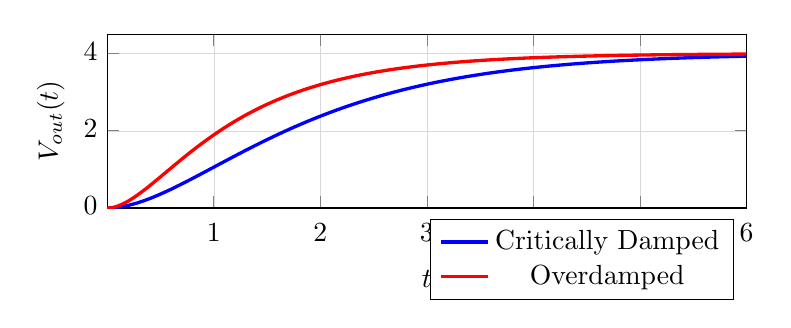
\begin{tikzpicture}[
      declare function={
        cd(\x)= -4*\x * exp(-\x) - 4* exp(-\x) + 4;
        od(\x)= 2*exp(-3*\x) - 6*exp(-\x) + 4;
      }
  ]

  \begin{axis}[
    typeset ticklabels with strut,
    ymin=0, ymax=4.5, ylabel=$V_{out}(t)$, xlabel=$t$,
    xmin = 0, xmax = 6, xtick = {1,2,3,4,5,6}, domain=0:6, 
    grid=both, grid style={line width=.1pt, draw=gray!30},
    width=\textwidth * 0.8,
    height=\textwidth / 3.2,
    legend style ={yshift=-2.3cm},
    samples = 1000
  ]
  \addplot [blue,very thick] {cd(x)};
  \addlegendentry{Critically Damped}
  \addplot [red,very thick] {od(x)};
  \addlegendentry{Overdamped}
  \end{axis}
  \end{tikzpicture}
  \end{figure}

  This was because, the eigenvalues picked for the capacitor were picked to ease calculation.
  The critically damped case is defined to be the case in which the response reaches the steady state, the quickest.
  However, notice that since we increased the value of our capacitor, it will take longer for the capacitor to fully charge.

  The scenario in which $R = \SI{4}{\ohm}, L = \SI{1}{\henry}, C = \SI{1/3}{\farad},$ is a different scenario, since we have changed the natural frequency $\omega_{0} = \frac{1}{\sqrt{LC}}$ of our circuit as opposed to the damping ratio. 
  Therefore, when we modify our components to reach critical damping, we can only modify our damping ratio or the value of the resistor.
  The critically damped situation for the first scenario is plotted below in which $R = \SI{4}{\ohm}, L = \SI{1}{\henry}, C = \SI{1/3}{\farad},$ 

  \begin{figure}[!h]
  \centering
  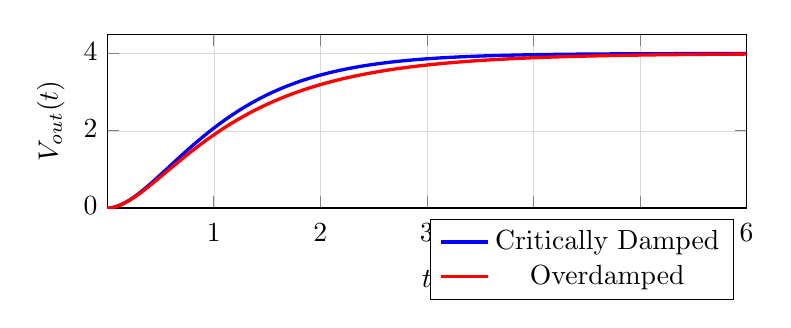
\begin{tikzpicture}[
    declare function={
      cd(\x)= 4*exp(-sqrt(3) * \x) * (-sqrt(3) * \x + exp(sqrt(3) * (\x)) - 1);
      od(\x)= 2*exp(-3*\x) - 6*exp(-\x) + 4;
    }
  ]
  \begin{axis}[
    typeset ticklabels with strut,
    ymin=0, ymax=4.5, ylabel=$V_{out}(t)$, xlabel=$t$,
    xmin = 0, xmax = 6, xtick = {1,2,3,4,5,6}, domain=0:6, 
    grid=both, grid style={line width=.1pt, draw=gray!30},
    width=\textwidth * 0.8,
    height=\textwidth / 3.2,
    legend style ={yshift=-2.3cm},
    samples = 1000
  ]
  \addplot [blue,very thick] {cd(x)};
  \addlegendentry{Critically Damped}
  \addplot [red,very thick] {od(x)};
  \addlegendentry{Overdamped}
  \end{axis}
  \end{tikzpicture}
  \end{figure}
  
  }
\end{enumerate}